% Options for packages loaded elsewhere
\PassOptionsToPackage{unicode}{hyperref}
\PassOptionsToPackage{hyphens}{url}
%
\documentclass[
  ignorenonframetext,
  aspectratio=1610,
]{beamer}
\usepackage{pgfpages}
\setbeamertemplate{caption}[numbered]
\setbeamertemplate{caption label separator}{: }
\setbeamercolor{caption name}{fg=normal text.fg}
\beamertemplatenavigationsymbolsempty
% Prevent slide breaks in the middle of a paragraph
\widowpenalties 1 10000
\raggedbottom
\setbeamertemplate{part page}{
  \centering
  \begin{beamercolorbox}[sep=16pt,center]{part title}
    \usebeamerfont{part title}\insertpart\par
  \end{beamercolorbox}
}
\setbeamertemplate{section page}{
  \centering
  \begin{beamercolorbox}[sep=12pt,center]{part title}
    \usebeamerfont{section title}\insertsection\par
  \end{beamercolorbox}
}
\setbeamertemplate{subsection page}{
  \centering
  \begin{beamercolorbox}[sep=8pt,center]{part title}
    \usebeamerfont{subsection title}\insertsubsection\par
  \end{beamercolorbox}
}
\AtBeginPart{
  \frame{\partpage}
}
\AtBeginSection{
  \ifbibliography
  \else
    \frame{\sectionpage}
  \fi
}
\AtBeginSubsection{
  \frame{\subsectionpage}
}
\usepackage{amsmath,amssymb}
\usepackage{iftex}
\ifPDFTeX
  \usepackage[T1]{fontenc}
  \usepackage[utf8]{inputenc}
  \usepackage{textcomp} % provide euro and other symbols
\else % if luatex or xetex
  \usepackage{unicode-math} % this also loads fontspec
  \defaultfontfeatures{Scale=MatchLowercase}
  \defaultfontfeatures[\rmfamily]{Ligatures=TeX,Scale=1}
\fi
\usepackage{lmodern}
\ifPDFTeX\else
  % xetex/luatex font selection
\fi
% Use upquote if available, for straight quotes in verbatim environments
\IfFileExists{upquote.sty}{\usepackage{upquote}}{}
\IfFileExists{microtype.sty}{% use microtype if available
  \usepackage[]{microtype}
  \UseMicrotypeSet[protrusion]{basicmath} % disable protrusion for tt fonts
}{}
\makeatletter
\@ifundefined{KOMAClassName}{% if non-KOMA class
  \IfFileExists{parskip.sty}{%
    \usepackage{parskip}
  }{% else
    \setlength{\parindent}{0pt}
    \setlength{\parskip}{6pt plus 2pt minus 1pt}}
}{% if KOMA class
  \KOMAoptions{parskip=half}}
\makeatother
\usepackage{xcolor}
\newif\ifbibliography
\usepackage{graphicx}
\makeatletter
\def\maxwidth{\ifdim\Gin@nat@width>\linewidth\linewidth\else\Gin@nat@width\fi}
\def\maxheight{\ifdim\Gin@nat@height>\textheight\textheight\else\Gin@nat@height\fi}
\makeatother
% Scale images if necessary, so that they will not overflow the page
% margins by default, and it is still possible to overwrite the defaults
% using explicit options in \includegraphics[width, height, ...]{}
\setkeys{Gin}{width=\maxwidth,height=\maxheight,keepaspectratio}
% Set default figure placement to htbp
\makeatletter
\def\fps@figure{htbp}
\makeatother
\setlength{\emergencystretch}{3em} % prevent overfull lines
\providecommand{\tightlist}{%
  \setlength{\itemsep}{0pt}\setlength{\parskip}{0pt}}
\setcounter{secnumdepth}{-\maxdimen} % remove section numbering
\ifLuaTeX
\usepackage[bidi=basic]{babel}
\else
\usepackage[bidi=default]{babel}
\fi
\babelprovide[main,import]{english}
% get rid of language-specific shorthands (see #6817):
\let\LanguageShortHands\languageshorthands
\def\languageshorthands#1{}
\usepackage{pgfpages}
\usepackage{pgfplots}
\usepackage{microtype}
\usepackage{tikz}
  \usetikzlibrary{positioning}
  \usetikzlibrary{arrows}
  \usetikzlibrary{graphs}

\definecolor{CTred}{RGB}{229,32,32}
\definecolor{CTgrey}{RGB}{153,153,153}

\usepackage{array}
\usepackage{dcolumn}
\newcolumntype{d}{D{.}{.}{-1}}
\usepackage{booktabs}
\usepackage{threeparttable}
\usepackage{emoji}
\usepackage{subcaption} % Subfigures and subcaptions

% colors: white text on 90% black background
\setbeamercolor{normal text}{fg=black,bg=white}

% light blue as a highlight color
\setbeamercolor*{structure}{fg=CTred}
\setbeamercolor{section title}{fg=CTred}
\setbeamercolor{alerted text}{use=structure,fg=CTred}
\setbeamercolor*{palette primary}{use=structure,fg=structure.fg}
\setbeamercolor*{palette secondary}{use=structure,fg=structure.fg!95!black}
\setbeamercolor*{palette tertiary}{use=structure,fg=structure.fg!90!black}
\setbeamercolor*{palette quaternary}{use=structure,fg=structure.fg!95!black,bg=black!80}

\setbeamercolor*{framesubtitle}{fg=white}


% use system fonts: here, Gill Sans
\usefonttheme{professionalfonts}
\setbeamerfont{quote}{shape=\upshape}

% eliminate silly beamer navigation line at bottom of slides
\setbeamertemplate{navigation symbols}{}
\setbeamertemplate{footline}[frame number]

% ensure text jusfication
\usepackage{ragged2e}
\justifying

% pandoc makes 2nd-lever headers into blocks, and this ensures justification
% in blocks too
\addtobeamertemplate{block begin}{}{\justifying}




\urlstyle{same}
\usepackage[overlay,absolute]{textpos}

\setbeamertemplate{items}[square]

\TPGrid[10 mm,8 mm]{9}{8}
% beamer's left and right margin is 10 mm. The top/bottom margin is ??
% or without a header ??
% the slide dimensions are 128 mm x 96 mm
% so the resulting \TPHorizModule = 12 mm and \TPVertModule = 10 mm

% uncomment if you want biblatex for citations on slides

% \usepackage{csquotes}
% \usepackage[notes,short,noibid,backend=biber]{biblatex-chicago}
% \bibliography{course.bib} 

\providecommand{\exhibit}[2]{\includegraphics[keepaspectratio, height=0.9\textheight, width=\textwidth]{assets/img/#1}\\ {\tiny #2}}

\providecommand{\smallcite}[1]{({\footnotesize #1})}
\ifLuaTeX
  \usepackage{selnolig}  % disable illegal ligatures
\fi
\IfFileExists{bookmark.sty}{\usepackage{bookmark}}{\usepackage{hyperref}}
\IfFileExists{xurl.sty}{\usepackage{xurl}}{} % add URL line breaks if available
\urlstyle{same}
\hypersetup{
  pdftitle={Success and geography: Evidence from open-source software},
  pdfauthor={Gábor Békés (CEU, HUN-REN KRTK, and CEPR),; Julian Hinz (Bielefeld University and Kiel Institute for the World Economy); Miklós Koren (CEU, HUN-REN KRTK, CEPR and CESifo),; Aaron Lohmann (Bielefeld University and Kiel Institute for the World Economy)},
  pdflang={en},
  hidelinks,
  pdfcreator={LaTeX via pandoc}}

\title{Success and geography: Evidence from open-source software}
\author{Gábor Békés (CEU, HUN-REN KRTK, and CEPR), \and Julian Hinz
(Bielefeld University and Kiel Institute for the World
Economy) \and Miklós Koren (CEU, HUN-REN KRTK, CEPR and
CESifo), \and Aaron Lohmann (Bielefeld University and Kiel Institute for
the World Economy)}
\date{April 20, 2024\footnote<.->{This work was funded by the European
  Union under the Horizon Europe grant 101061123. Views and opinions
  expressed are, however, those of the author(s) only and do not
  necessarily reflect those of the European Union or the European
  Commission. Neither the European Union nor the granting authority can
  be held responsible for them.}}

\begin{document}
\frame{\titlepage}

\section{Introduction}\label{introduction}

\begin{frame}{Research question}
\protect\hypertarget{research-question}{}
\begin{itemize}
\tightlist
\item
  How and where is open source software developed?
\item
  Can spatially dispersed developers produce quality software?
\end{itemize}
\end{frame}

\section{GitHub poll}\label{github-poll}

\section{\texorpdfstring{\texttt{if\ (poll\ ==\ "no")\ \{}}{if (poll == "no") \{}}\label{if-poll-no}

\begin{frame}{Why Open Source Software (OSS)?}
\protect\hypertarget{why-open-source-software-oss}{}
\begin{block}{OSS is huge}
\protect\hypertarget{oss-is-huge}{}
\begin{itemize}
\tightlist
\item
  Software industry -- 1\% of global GDP
\item
  90+\% of software has open source components
\end{itemize}
\end{block}

\begin{block}{OSS is everywhere}
\protect\hypertarget{oss-is-everywhere}{}
OSS plays an important roles in

\begin{itemize}
\tightlist
\item
  Websites (PHP, JavaScript)
\item
  Operating systems (Linux, Android)
\item
  Data (R Tidyverse, Python Pandas, Julia)
\item
  Machine Learning and AI (PyTorch, LLaMA)
\end{itemize}
\end{block}

\begin{block}{OSS is observable}
\protect\hypertarget{oss-is-observable}{}
\end{block}
\end{frame}

\begin{frame}{Collaboration is done mostly online}
\protect\hypertarget{collaboration-is-done-mostly-online}{}
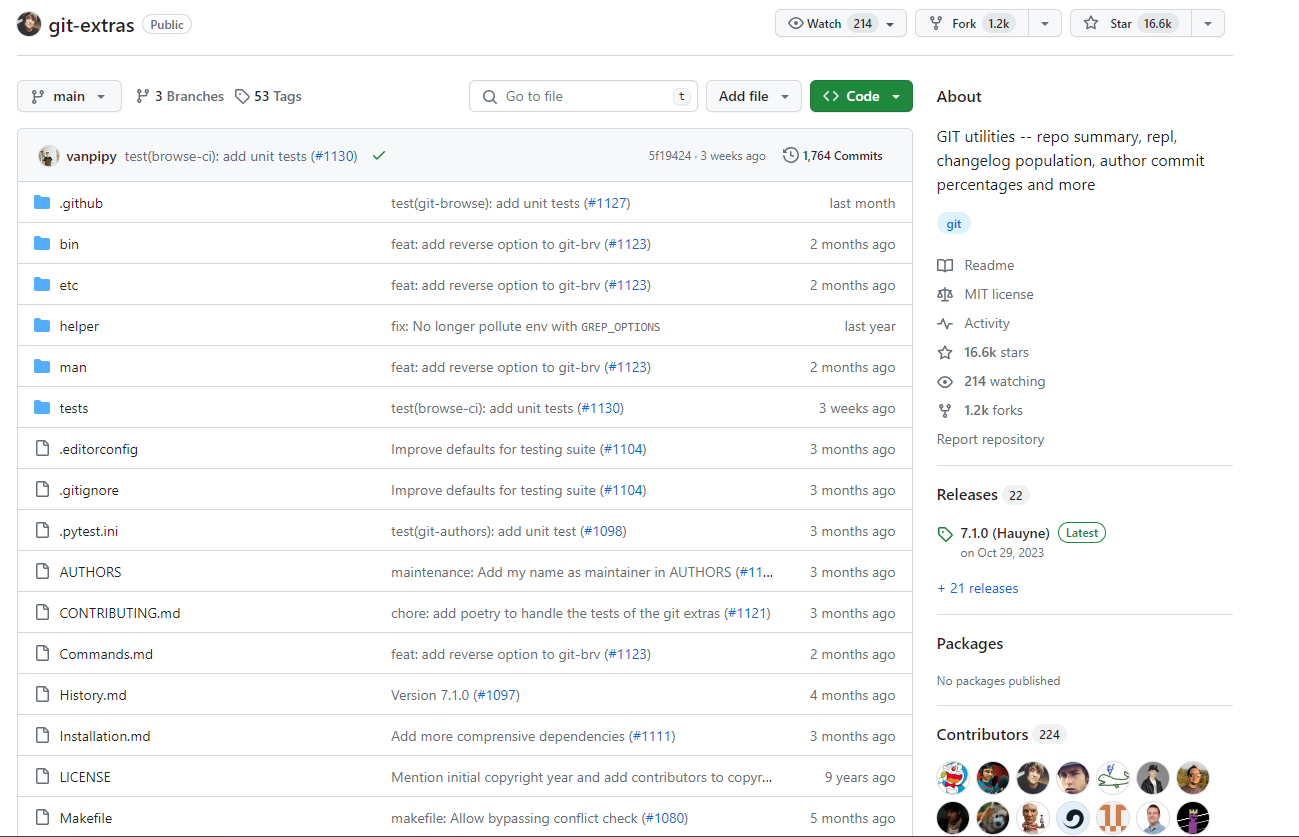
\includegraphics{images/github-example.png}
\end{frame}

\begin{frame}{Collaboration is done mostly online}
\protect\hypertarget{collaboration-is-done-mostly-online-1}{}
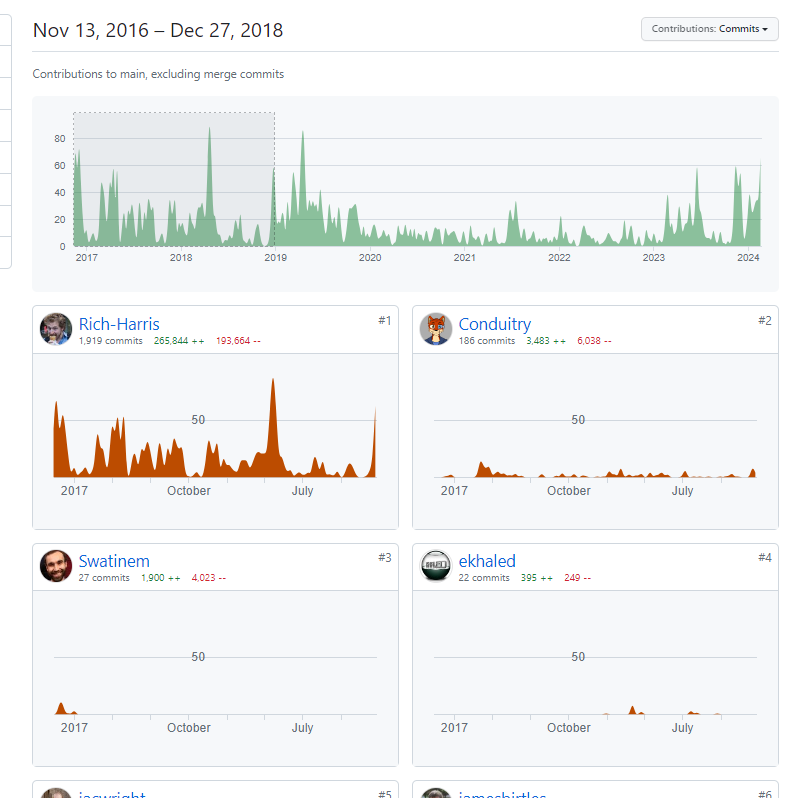
\includegraphics{images/collab-example-2017-19.png}
\end{frame}

\begin{frame}[fragile]{Open Source vocabulary}
\protect\hypertarget{open-source-vocabulary}{}
\texttt{Package}: A unit of software, provision of a (bundle of)
functionality

\texttt{Project}: A software project offering solution to a use case.
Typically one package, but may be more.

\texttt{Repository}: A storage for one project (what we observe)

\texttt{Commit}: The smallest unit of contribution

\texttt{Git}: Distributed version control system for software projects

\texttt{GitHub}: A platform to collaboratively work on software projects

\texttt{Dependency}: An imported package that provides a functionality
\end{frame}

\section{\texorpdfstring{\texttt{\}}}{\}}}\label{section}

\begin{frame}{Related literature}
\protect\hypertarget{related-literature}{}
\begin{itemize}
\tightlist
\item
  \textbf{Geographical Distance / Network formation / Agglomeration}:
  {[}@chaney2014network{]} {[}@bernard2019production{]}
  {[}@davis2019spatial{]} {[}@BaileyGuptaHillenbrandEtAl2021{]},
  {[}@Atkin\_2022\_F2F{]}
\item
  \textbf{Gravity:} \textbf{Digital:} {[}@blum2006does{]}
  {[}@anderson2018dark{]}
\item
  \textbf{Frictions in services:} {[}@stein2007longitude{]}
  {[}@bahar2020hardships{]}
\item
  \textbf{Patents and science}: {[}@BircanJavorcikPauly2021{]},
  {[}@head\_li\_minondo\_math\_2019{]}, {[}@jaffe1993geographic{]},
  Singh (2008) {[}@AlShebli\_nature\_2018{]}, {[}@Li2014-patents-eer{]}
\item
  \textbf{OSS}: {[}@lerner2002some{]} , {[}@Laurentsyeva:2019{]}
  {[}@Wachs\_etal\_2022{]} {[}@fackler\_hofmann\_laurentsyeva\_2023{]}
\end{itemize}
\end{frame}

\begin{frame}{Data}
\protect\hypertarget{data}{}
\begin{block}{GitHub}
\protect\hypertarget{github}{}
Snapshot of all public repositories on GitHub on 2019-06-01. Six largest
languages: JavaScript, Python, Java, Ruby, PHP, and C++. Drop smallest
and largest projects. 4.4m projects, 2.7m users. Self-reported location
for about 1/3 os users.
\end{block}

\begin{block}{libraries.io}
\protect\hypertarget{libraries.io}{}
Dependency data for projects on major package managers (npm, PyPI,
Maven, RubyGems, etc).
\end{block}
\end{frame}

\begin{frame}{Developer density around the globe}
\protect\hypertarget{developer-density-around-the-globe}{}
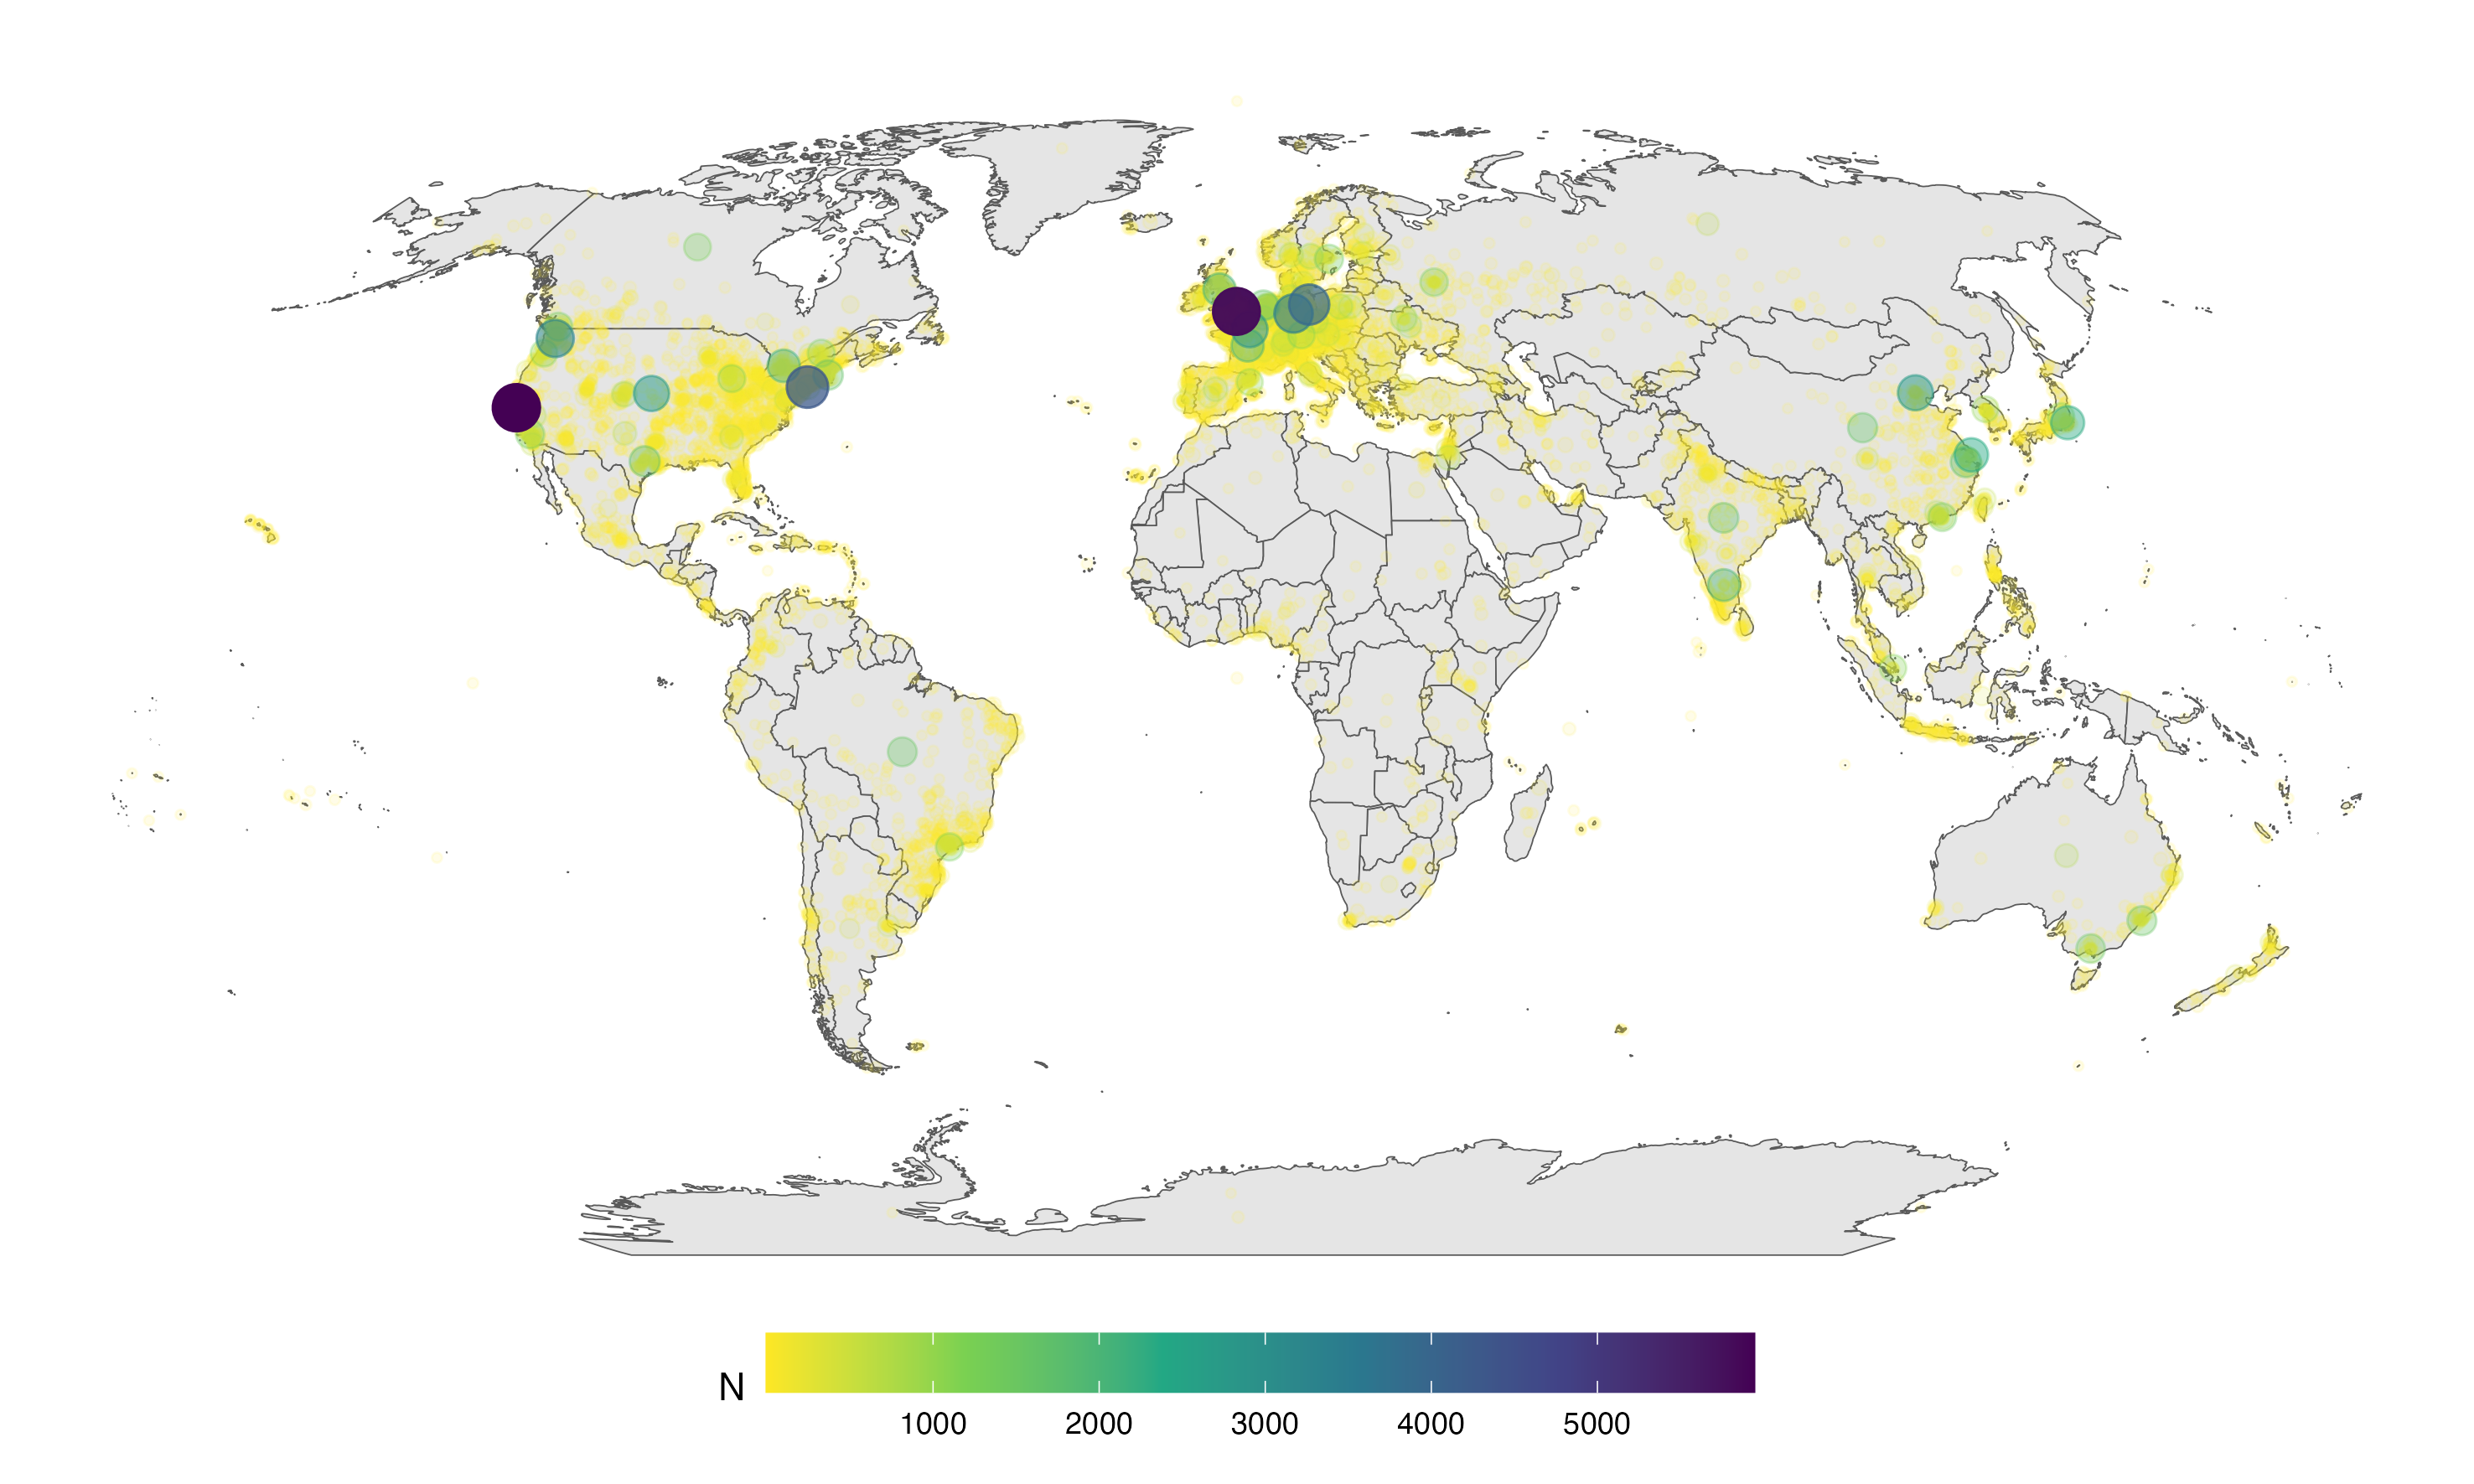
\includegraphics{figures/map_developers.png}
\end{frame}

\section{Descriptives}\label{descriptives}

\begin{frame}{Project size and popularity}
\protect\hypertarget{project-size-and-popularity}{}
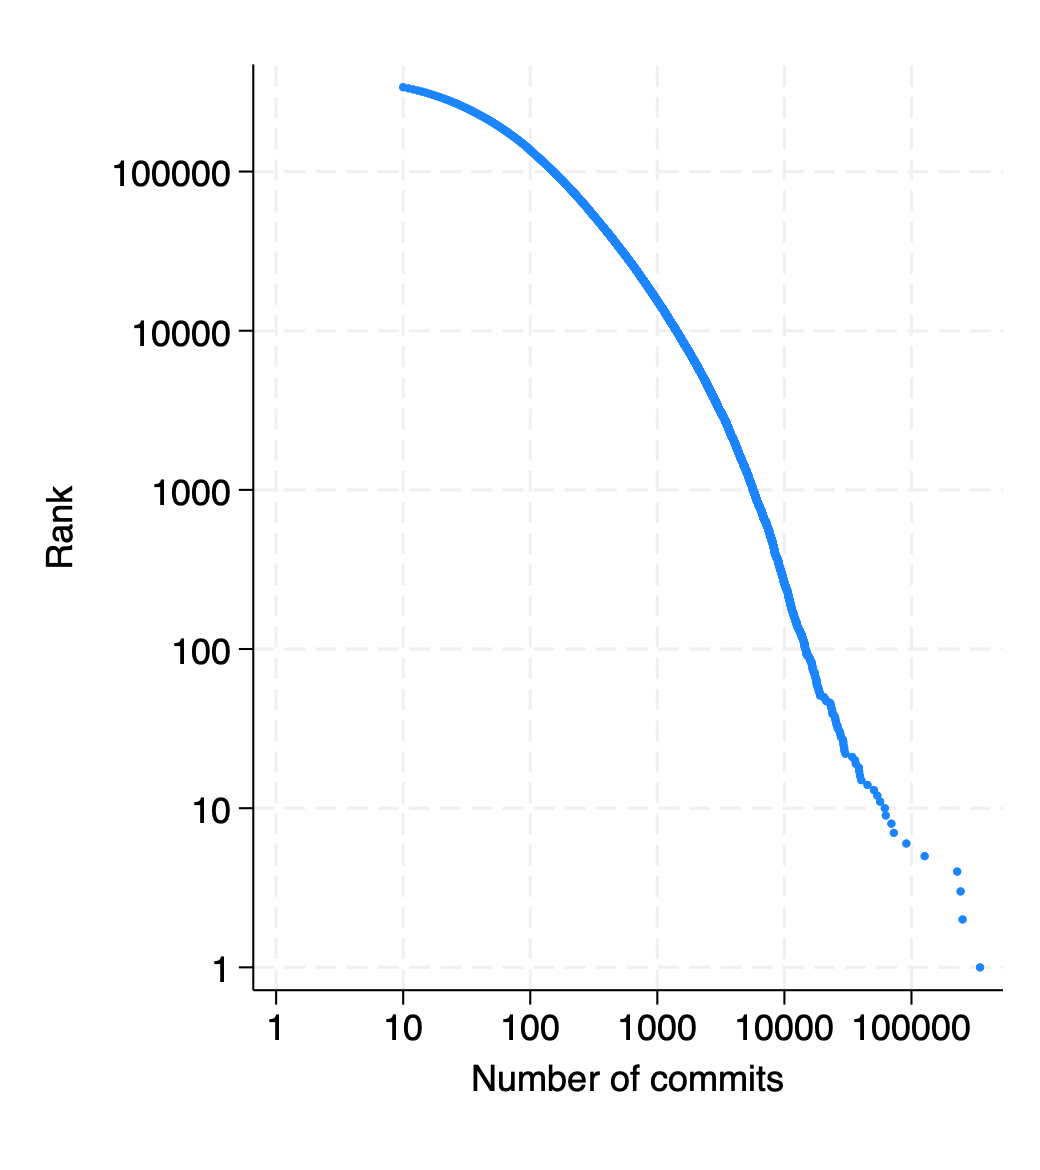
\includegraphics[width=7cm,height=\textheight]{figures/commits_rank.png}
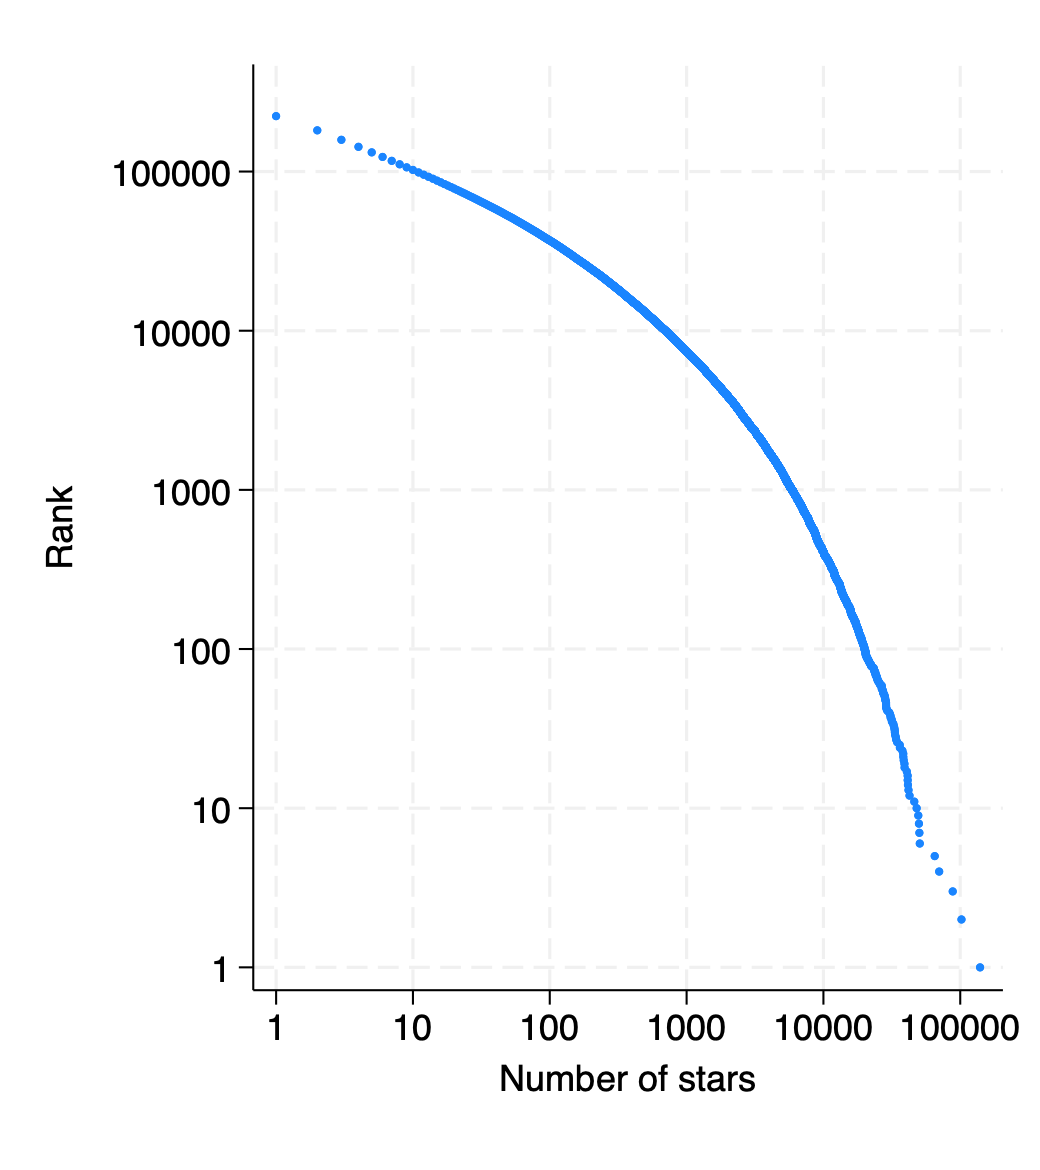
\includegraphics[width=7cm,height=\textheight]{figures/stars_rank.png}
\end{frame}

\begin{frame}{Team size and total developer effort}
\protect\hypertarget{team-size-and-total-developer-effort}{}
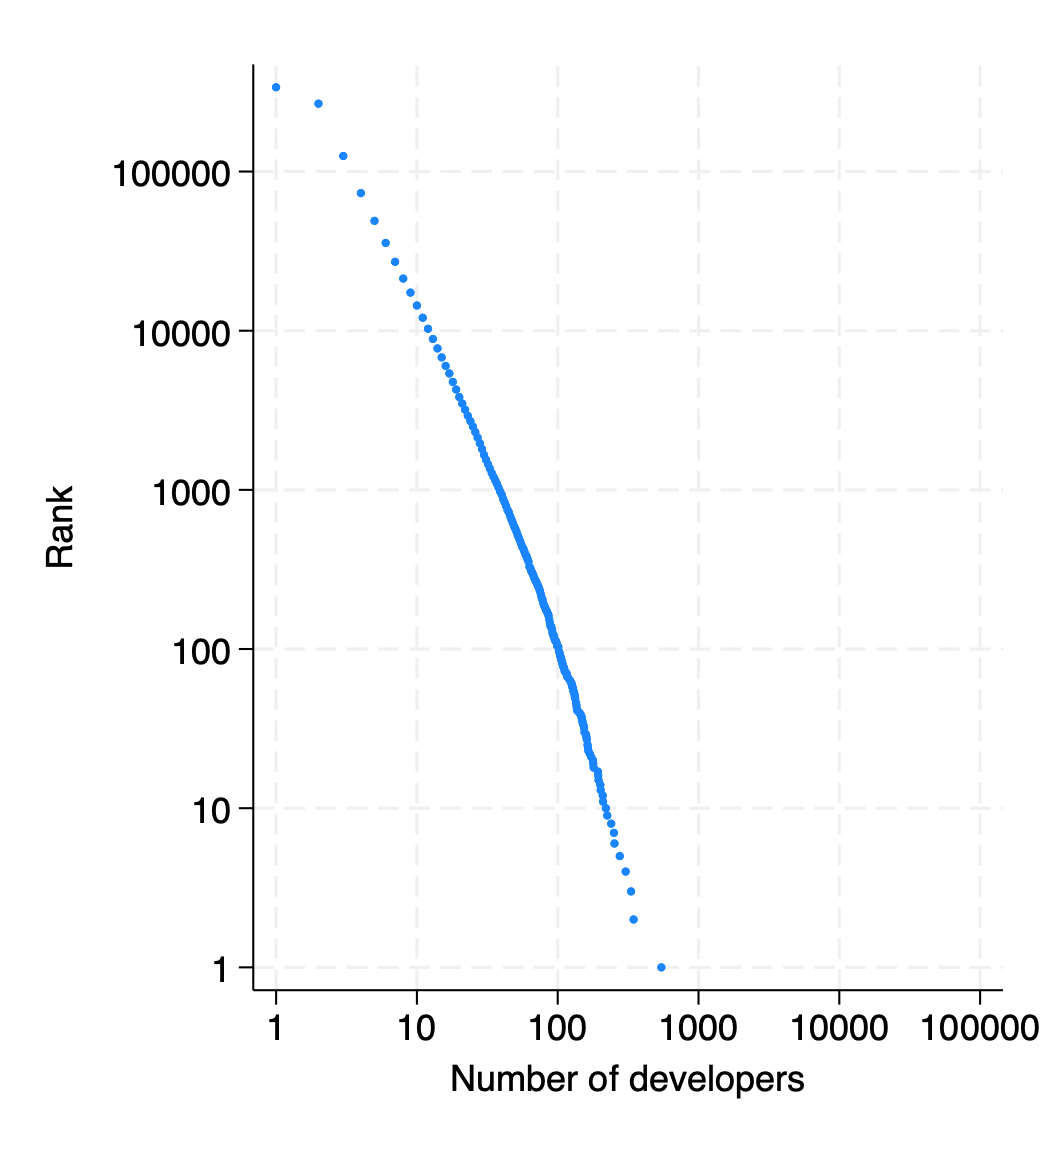
\includegraphics[width=7cm,height=\textheight]{figures/developers_rank.png}
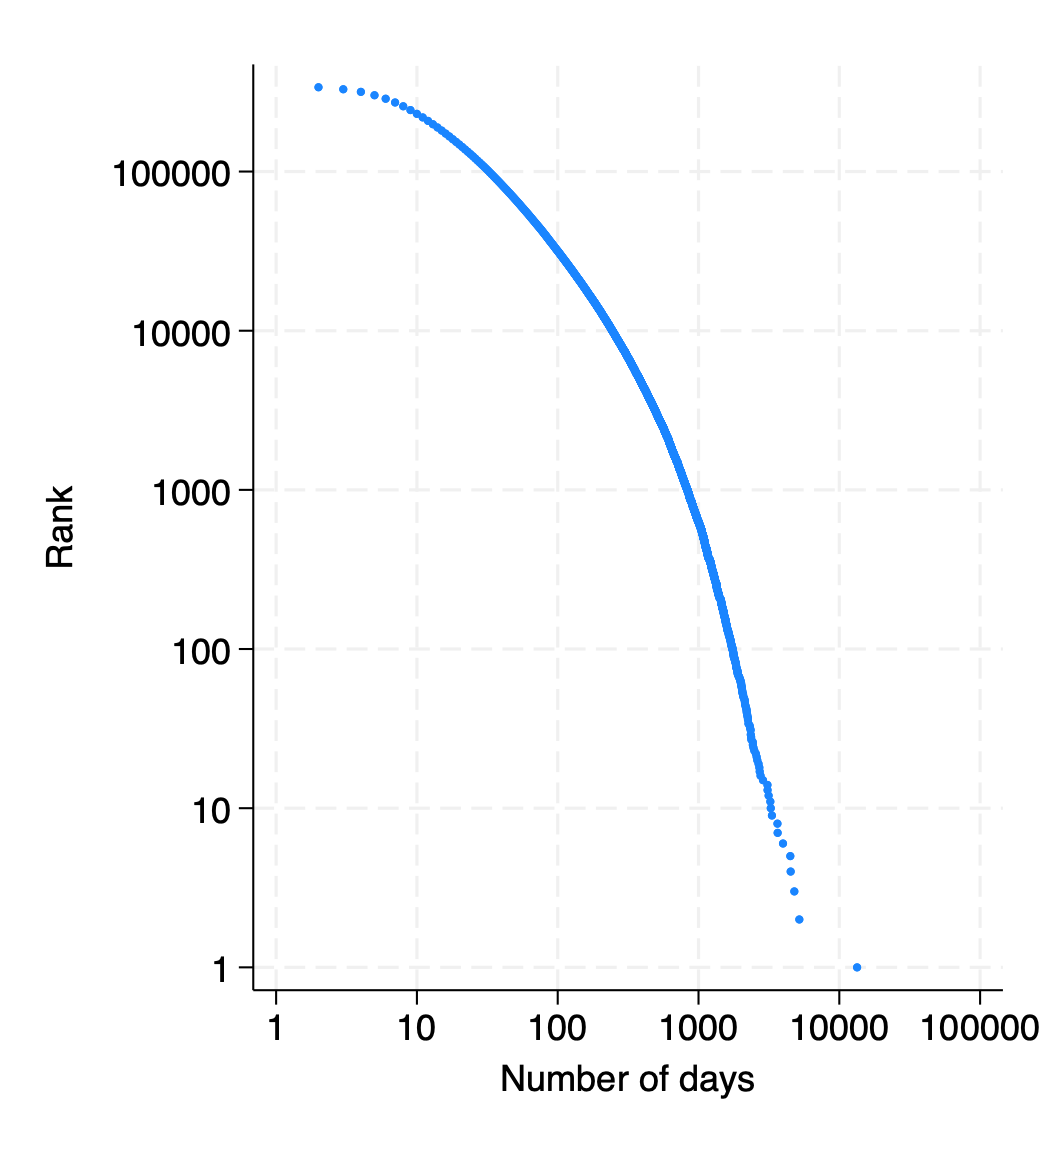
\includegraphics[width=7cm,height=\textheight]{figures/days_rank.png}
\end{frame}

\begin{frame}{Geographic diversity of teams}
\protect\hypertarget{geographic-diversity-of-teams}{}
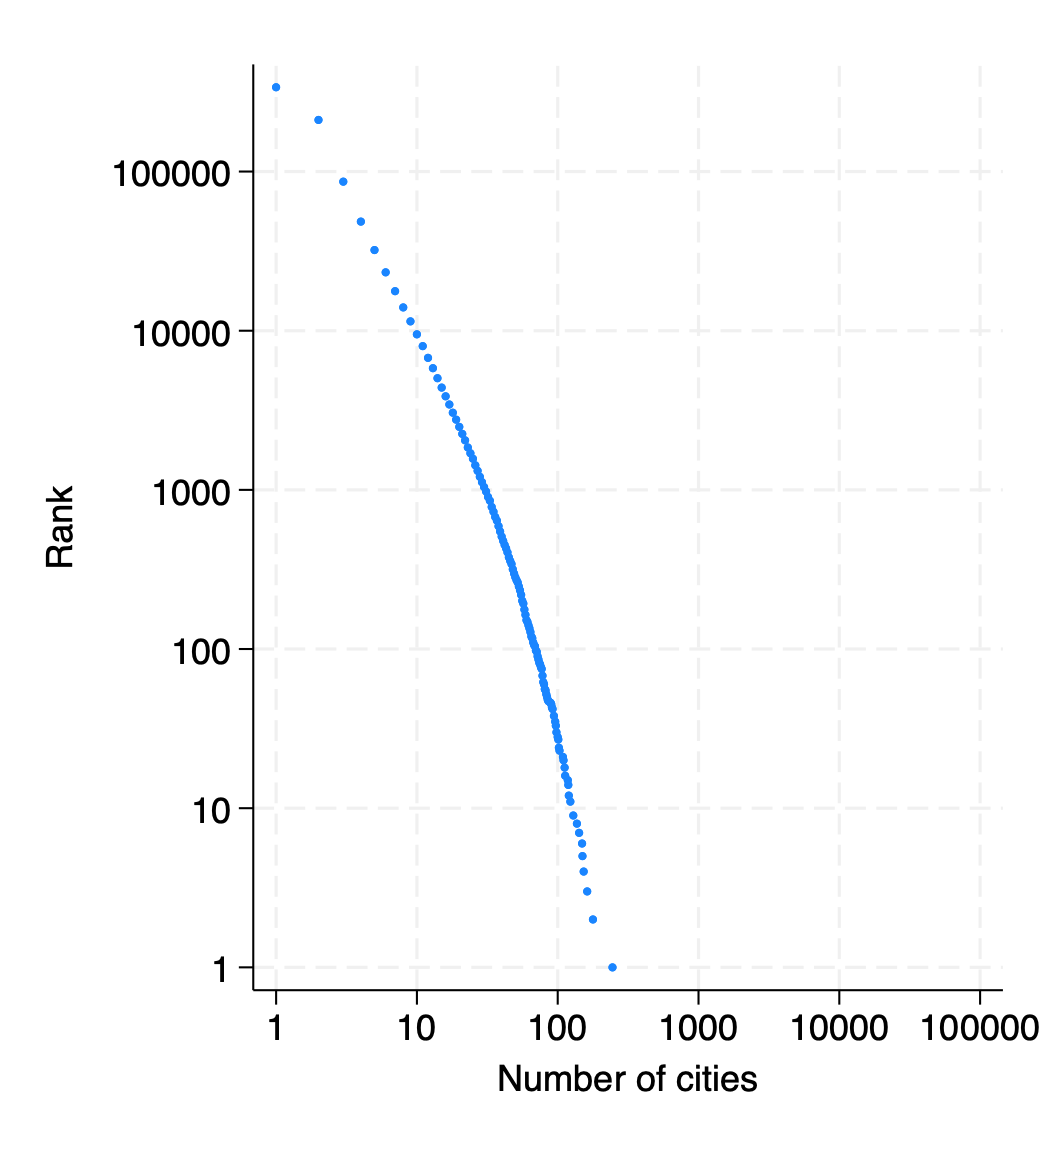
\includegraphics[width=7cm,height=\textheight]{figures/cities_rank.png}
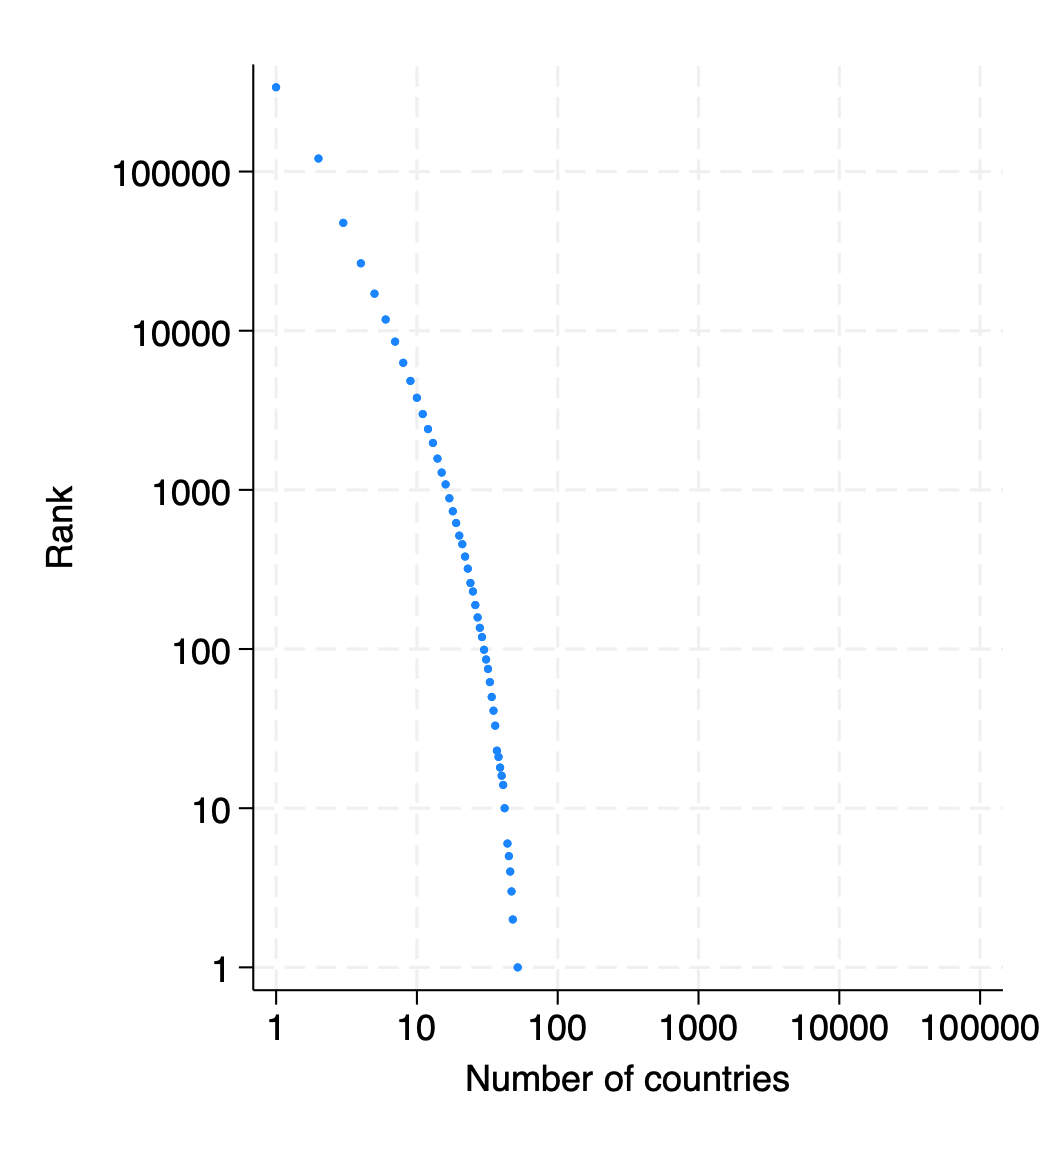
\includegraphics[width=7cm,height=\textheight]{figures/countries_rank.png}
\end{frame}

\begin{frame}{Collaboration across cities is mostly North-North}
\protect\hypertarget{collaboration-across-cities-is-mostly-north-north}{}
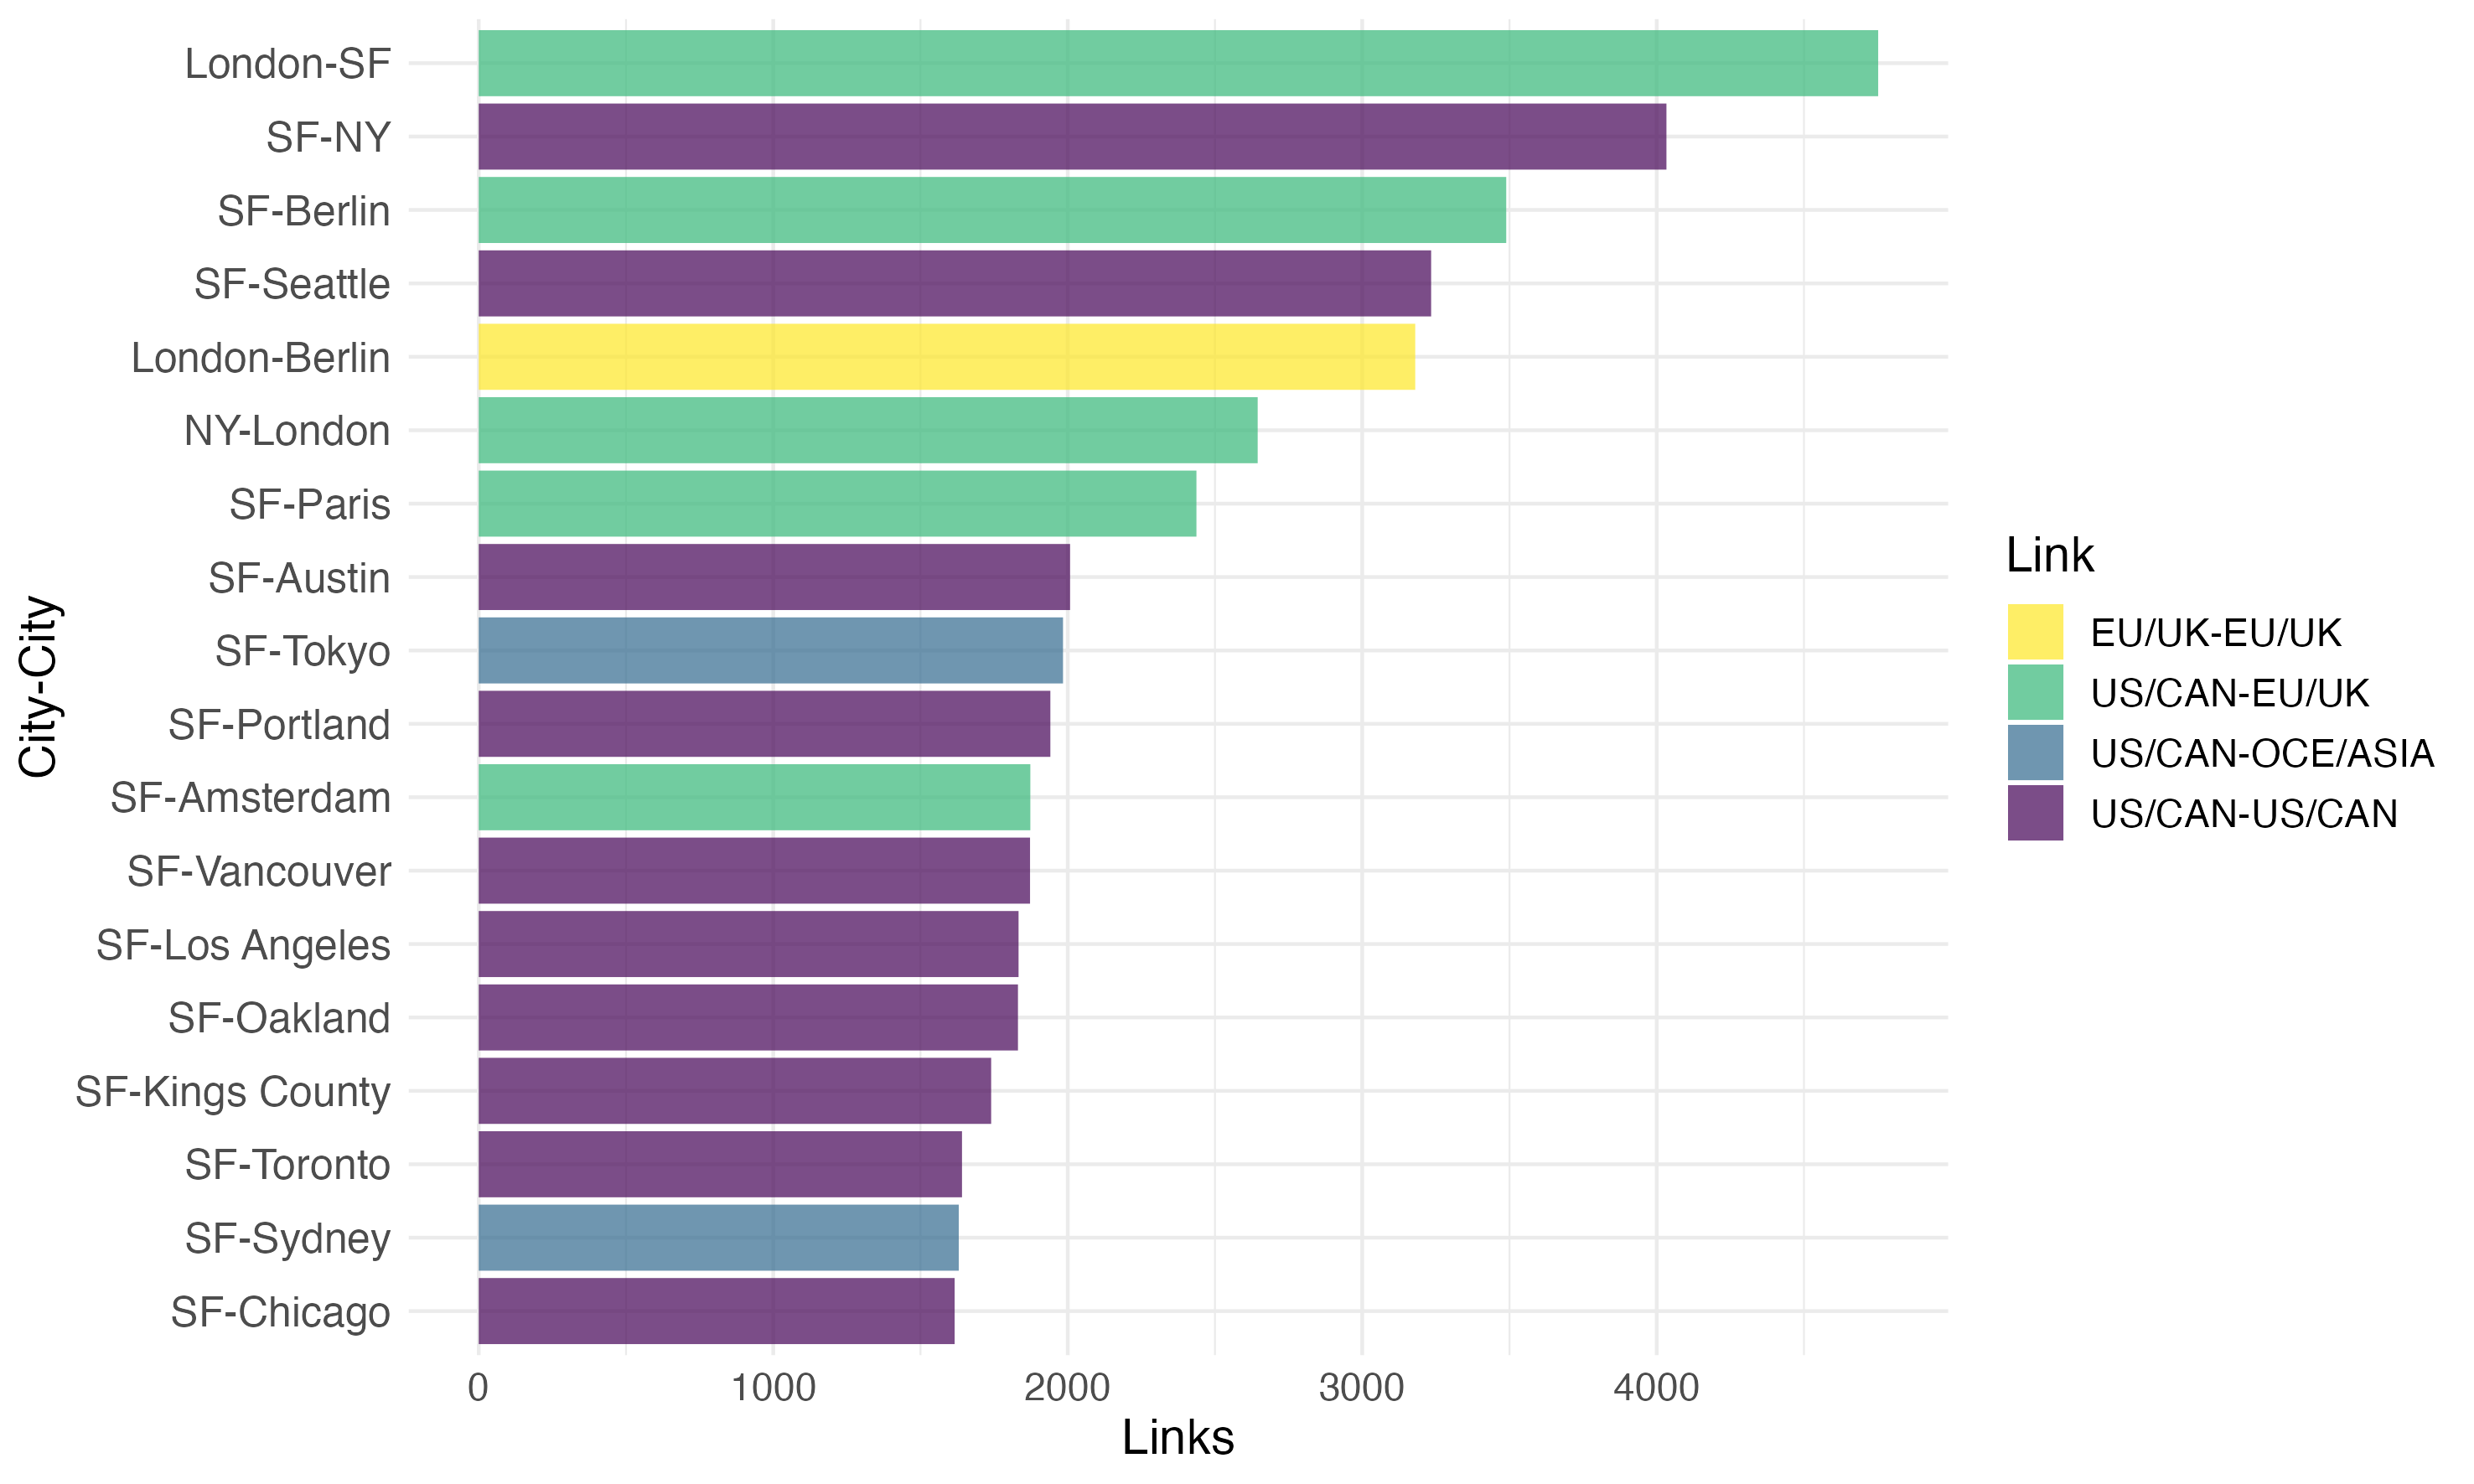
\includegraphics{figures/most_linked_city_pairs.png}

Most frequent city-pairs for repos developed from 2 cities
\end{frame}

\section{Collaboration}\label{collaboration}

\begin{frame}{Measuring collalboration and dependencies}
\protect\hypertarget{measuring-collalboration-and-dependencies}{}
\begin{figure}
    \begin{subfigure}{0.5\textwidth}
        \centering
        \begin{tikzpicture}[scale=0.9]
            % Nodes and arrows for the first figure
            \node[circle, draw] (A) at (0,2) {A};
            \node[circle, draw] (B) at (4,2) {B};
            \node[circle, draw] (C) at (4,0) {C};
            \node[rectangle, draw, minimum width=2cm, minimum height=1cm] (repo) at (0,0) {Repo}; % Adjust the width and height as needed

            \draw[->] (A) -- (repo);
            \draw[->] (B) -- (repo);
            \draw[->] (C) -- (repo);
        \end{tikzpicture}
        \caption{Developers committing to a repository.}
    \end{subfigure}%
    \begin{subfigure}{0.5\textwidth}
        \centering
        \begin{tikzpicture}
            % Nodes and lines for the first figure
            \node[draw, circle, minimum size=1cm] (A) at (0,1.5) {A};
            \node[draw, circle, minimum size=1cm] (B) at (0,0) {B};
            \node[draw, rectangle, minimum width=1.5cm, minimum height=1cm] (Repo1) at (0,-1.5) {Repo 1};

            \node[draw, circle, minimum size=1cm] (C) at (3,1.5) {C};
            \node[draw, circle, minimum size=1cm] (D) at (3,0) {D};
            \node[draw, rectangle, minimum width=1.5cm, minimum height=1cm] (Repo2) at (3,-1.5) {Repo 2};

            \draw[solid] (1.5,-1.5) -- (1.5,2.5);
            \draw[->] (Repo1.east) -- (Repo2.west);
        \end{tikzpicture}
        \caption{Dependency of repository 1 on repository 2 with the respective developers.}
    \end{subfigure}%
\end{figure}
\end{frame}

\begin{frame}{Multiplexing}
\protect\hypertarget{multiplexing}{}
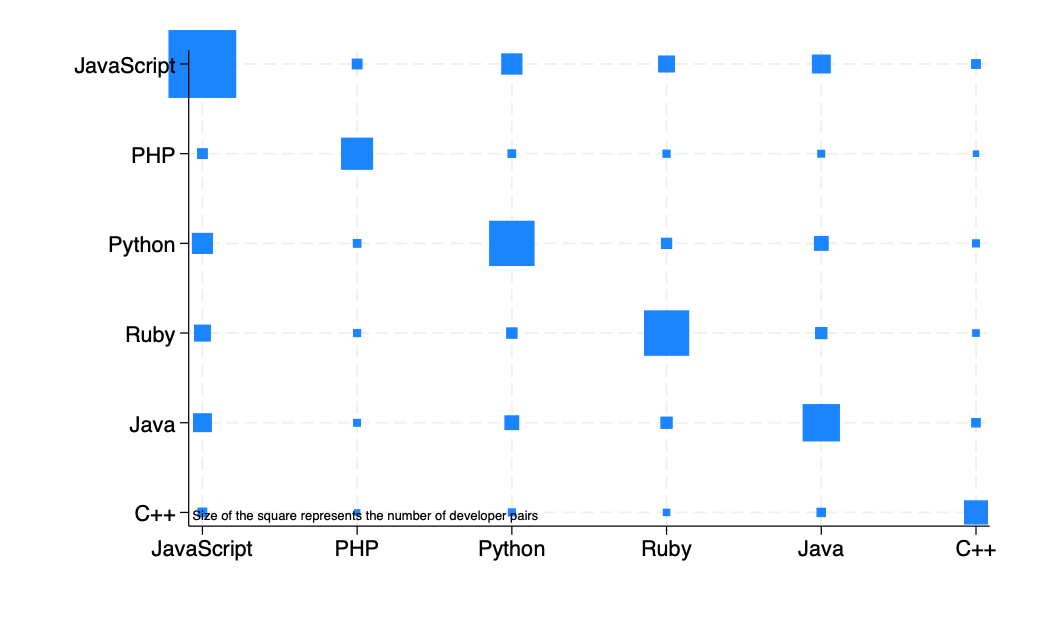
\includegraphics{figures/language_matrix.png}
\end{frame}

\begin{frame}{Multiplexing}
\protect\hypertarget{multiplexing-1}{}
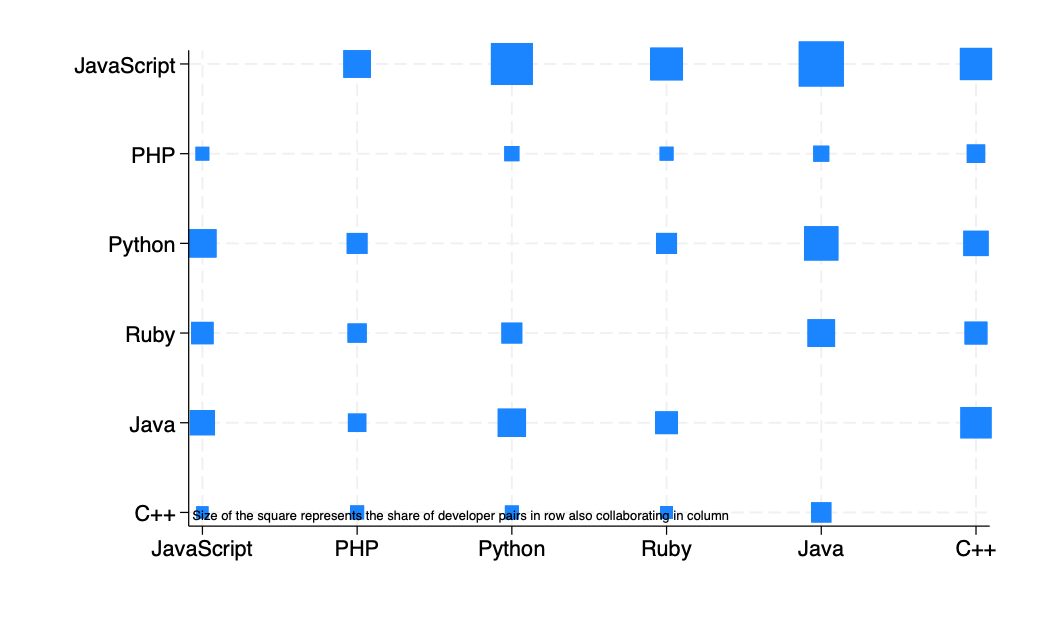
\includegraphics{figures/language_matrix_share.png}
\end{frame}

\begin{frame}{Some work is done within organizations}
\protect\hypertarget{some-work-is-done-within-organizations}{}
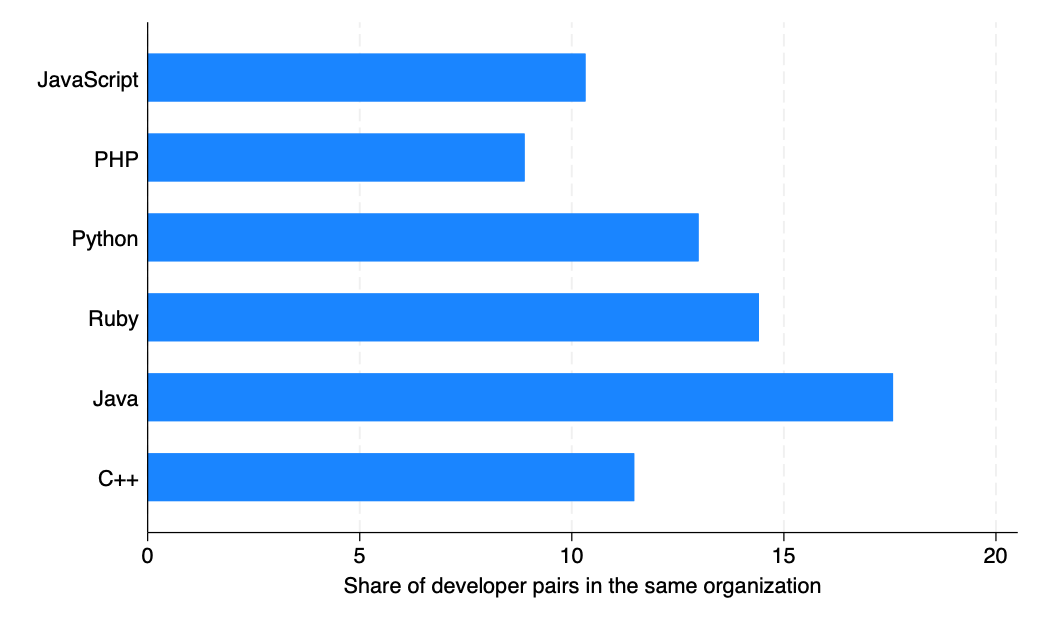
\includegraphics{figures/organization_share.png}
\end{frame}

\section{Collaboration in space}\label{collaboration-in-space}

\begin{frame}{Gravity model of collaboration}
\protect\hypertarget{gravity-model-of-collaboration}{}
Developer \(i\) and \(j\) collaborate with probability \[
\Pr(\text{Collaboration}_{ij}) = \exp(\alpha_i + \beta_j -\gamma\times\text{distance}_{ij})
\] Aggregate across city pairs \(d\) and \(o\): \[
E(N_{do}) = \exp(\tilde\alpha_d + \tilde\beta_o -\gamma\times\text{distance}_{do})
\] Estimate this with Poisson maximum likelihood.
\end{frame}

\begin{frame}{Four margins of collaboration}
\protect\hypertarget{four-margins-of-collaboration}{}
\begin{enumerate}
\tightlist
\item
  Committing to the same project
\item
  Commenting on the same issue
\item
  Editor rights on the same project
\item
  Members of the same organization
\end{enumerate}
\end{frame}

\begin{frame}{Gravity model of the developer-to-developer network}
\protect\hypertarget{gravity-model-of-the-developer-to-developer-network}{}
\begin{tabular}{lcccc} \hline
 & (1) & (2) & (3) & (4) \\
VARIABLES & commits & comments & editors & organizations \\ \hline
 &  &  &  &  \\
Distance (log km) & -0.143*** & -0.107*** & -0.277*** & -0.183*** \\
 & (0.0129) & (0.0139) & (0.0178) & (0.0313) \\
Same country (dummy) & 0.519*** & 0.584*** & 1.058*** & 0.706*** \\
 & (0.0528) & (0.107) & (0.0894) & (0.135) \\
Same city (dummy) & 0.846*** & 0.433*** & 0.856*** & 0.350** \\
 & (0.0863) & (0.0587) & (0.0924) & (0.154) \\
 &  &  &  &  \\
 Observations & 498,472 & 781,201 & 139,464 & 408,094 \\ \hline
\multicolumn{5}{c}{ Robust standard errors in parentheses} \\
\multicolumn{5}{c}{ *** p$<$0.01, ** p$<$0.05, * p$<$0.1} \\
\end{tabular}

\end{frame}

\begin{frame}{Odds ratios of collaboration}
\protect\hypertarget{odds-ratios-of-collaboration}{}
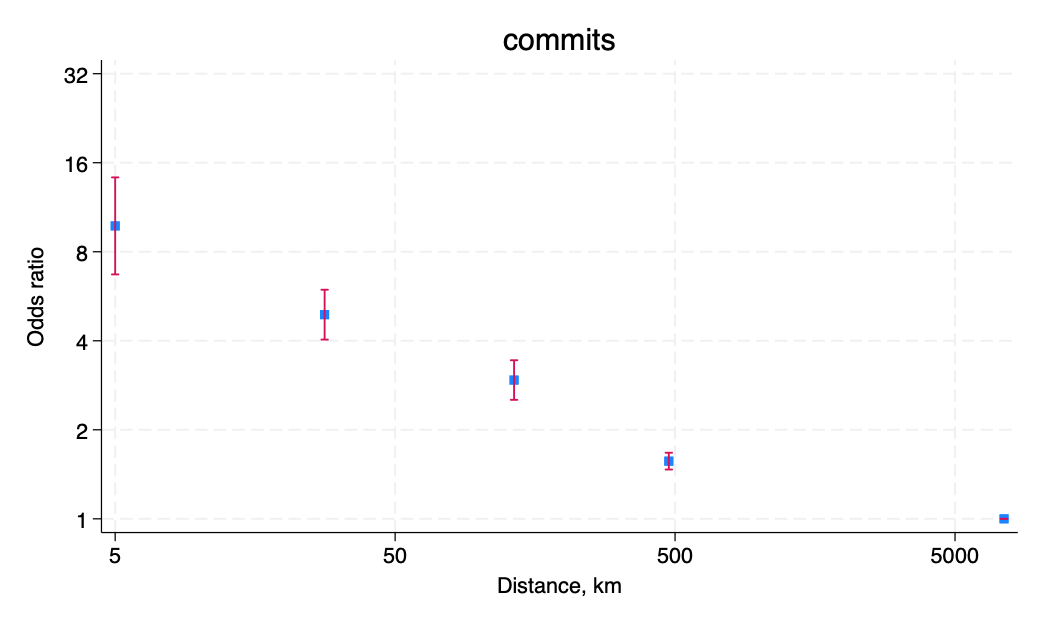
\includegraphics{figures/commits_gravity.png}
\end{frame}

\begin{frame}{Editor rights are most localized}
\protect\hypertarget{editor-rights-are-most-localized}{}
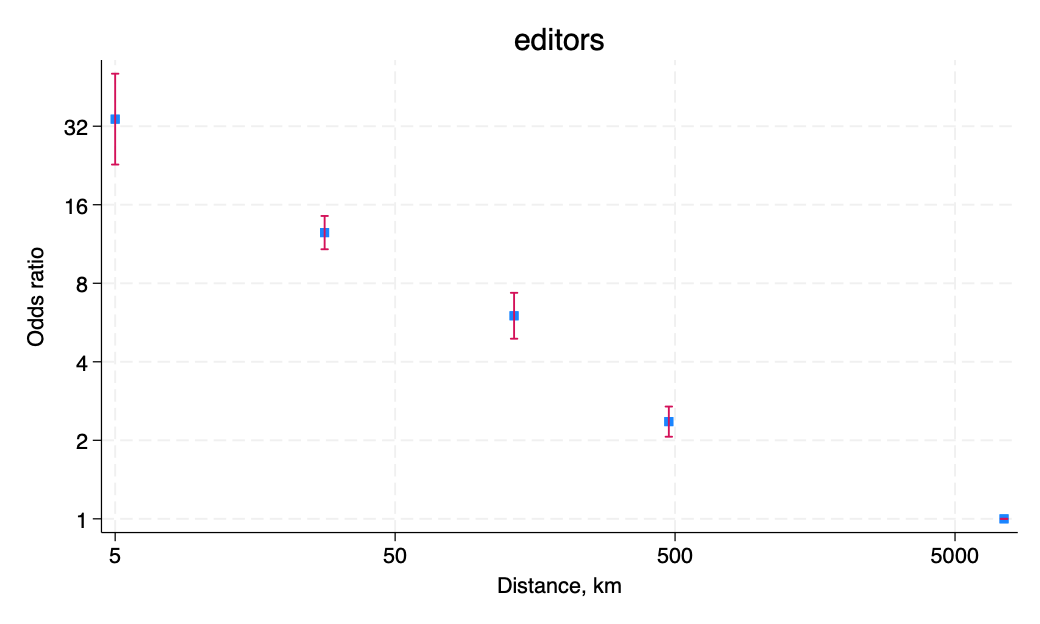
\includegraphics{figures/editors_gravity.png}
\end{frame}

\begin{frame}{Small differences across languages}
\protect\hypertarget{small-differences-across-languages}{}
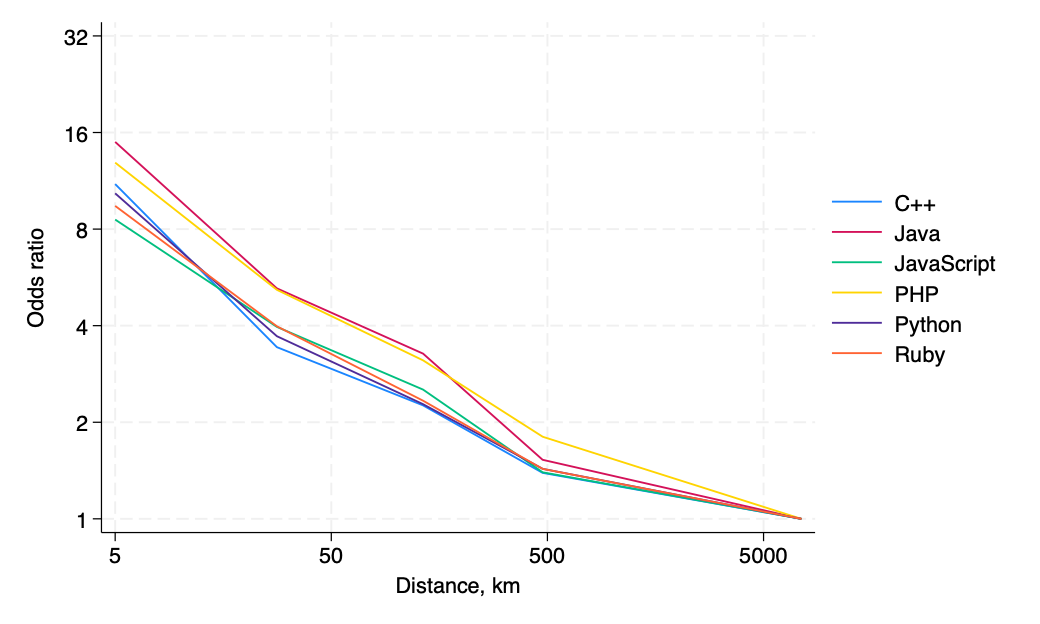
\includegraphics{figures/commits_by_language.png}
\end{frame}

\section{Success}\label{success}

\begin{frame}{Spatial diversity reduces amount of work}
\protect\hypertarget{spatial-diversity-reduces-amount-of-work}{}
\hspace*{-2em}\begin{tabular}{lcccc} \hline
 & (1) & (2) & (3) & (4) \\
VARIABLES & n\_commits & n\_commits & n\_days & n\_days \\ \hline
 &  &  &  &  \\
avg\_ln\_distance & 0.0409*** &  & 0.0384*** &  \\
 & (0.00416) &  & (0.00271) &  \\
ln\_n\_cities & -0.159*** &  & -0.218*** &  \\
 & (0.0302) &  & (0.0184) &  \\
ln\_n\_countries & -0.244*** &  & -0.212*** &  \\
 & (0.0231) &  & (0.0111) &  \\
ln\_n\_developers & 1.241*** & 0.935*** & 1.257*** & 0.929*** \\
 & (0.0296) & (0.0161) & (0.0171) & (0.00639) \\
share\_organization &  & -0.236*** &  & -0.0602*** \\
 &  & (0.0314) &  & (0.00921) \\
share\_different\_cities &  & 0.0534** &  & -0.0184* \\
 &  & (0.0255) &  & (0.0103) \\
share\_different\_countries &  & -0.124*** &  & -0.0955*** \\
 &  & (0.0234) &  & (0.0110) \\
 &  &  &  &  \\
 Observations & 267,086 & 267,086 & 267,086 & 267,086 \\ \hline
\multicolumn{5}{c}{ Robust standard errors in parentheses} \\
\multicolumn{5}{c}{ *** p$<$0.01, ** p$<$0.05, * p$<$0.1} \\
\end{tabular}

\end{frame}

\begin{frame}{Spatial diversity associated with higher quality}
\protect\hypertarget{spatial-diversity-associated-with-higher-quality}{}
\hspace*{-2em}\begin{tabular}{lcccc} \hline
 & (1) & (2) & (3) & (4) \\
VARIABLES & n\_stars & n\_stars & n\_downstream & n\_downstream \\ \hline
 &  &  &  &  \\
avg\_ln\_distance & 0.198*** &  & 0.299*** &  \\
 & (0.0114) &  & (0.0558) &  \\
ln\_n\_cities & 0.311*** &  & 1.817*** &  \\
 & (0.0780) &  & (0.344) &  \\
ln\_n\_countries & 0.364*** &  & 0.577*** &  \\
 & (0.0447) &  & (0.199) &  \\
ln\_n\_developers & 0.537*** & 1.020*** & -1.428*** & 0.683*** \\
 & (0.0797) & (0.0134) & (0.320) & (0.0409) \\
share\_organization &  & -1.769*** &  & 0.101 \\
 &  & (0.0446) &  & (0.147) \\
share\_different\_cities &  & 0.944*** &  & 4.144*** \\
 &  & (0.0534) &  & (0.768) \\
share\_different\_countries &  & 0.731*** &  & 1.217*** \\
 &  & (0.0406) &  & (0.184) \\
in\_libraries = o, &  &  & - & - \\
 &  &  &  &  \\
 &  &  &  &  \\
 Observations & 181,336 & 181,336 & 75,673 & 75,673 \\ \hline
\multicolumn{5}{c}{ Robust standard errors in parentheses} \\
\multicolumn{5}{c}{ *** p$<$0.01, ** p$<$0.05, * p$<$0.1} \\
\end{tabular}

\end{frame}

\end{document}
